\documentclass[1p]{elsarticle_modified}
%\bibliographystyle{elsarticle-num}

%\usepackage[colorlinks]{hyperref}
%\usepackage{abbrmath_seonhwa} %\Abb, \Ascr, \Acal ,\Abf, \Afrak
\usepackage{amsfonts}
\usepackage{amssymb}
\usepackage{amsmath}
\usepackage{amsthm}
\usepackage{scalefnt}
\usepackage{amsbsy}
\usepackage{kotex}
\usepackage{caption}
\usepackage{subfig}
\usepackage{color}
\usepackage{graphicx}
\usepackage{xcolor} %% white, black, red, green, blue, cyan, magenta, yellow
\usepackage{float}
\usepackage{setspace}
\usepackage{hyperref}

\usepackage{tikz}
\usetikzlibrary{arrows}

\usepackage{multirow}
\usepackage{array} % fixed length table
\usepackage{hhline}

%%%%%%%%%%%%%%%%%%%%%
\makeatletter
\renewcommand*\env@matrix[1][\arraystretch]{%
	\edef\arraystretch{#1}%
	\hskip -\arraycolsep
	\let\@ifnextchar\new@ifnextchar
	\array{*\c@MaxMatrixCols c}}
\makeatother %https://tex.stackexchange.com/questions/14071/how-can-i-increase-the-line-spacing-in-a-matrix
%%%%%%%%%%%%%%%

\usepackage[normalem]{ulem}

\newcommand{\msout}[1]{\ifmmode\text{\sout{\ensuremath{#1}}}\else\sout{#1}\fi}
%SOURCE: \msout is \stkout macro in https://tex.stackexchange.com/questions/20609/strikeout-in-math-mode

\newcommand{\cancel}[1]{
	\ifmmode
	{\color{red}\msout{#1}}
	\else
	{\color{red}\sout{#1}}
	\fi
}

\newcommand{\add}[1]{
	{\color{blue}\uwave{#1}}
}

\newcommand{\replace}[2]{
	\ifmmode
	{\color{red}\msout{#1}}{\color{blue}\uwave{#2}}
	\else
	{\color{red}\sout{#1}}{\color{blue}\uwave{#2}}
	\fi
}

\newcommand{\Sol}{\mathcal{S}} %segment
\newcommand{\D}{D} %diagram
\newcommand{\A}{\mathcal{A}} %arc


%%%%%%%%%%%%%%%%%%%%%%%%%%%%%5 test

\def\sl{\operatorname{\textup{SL}}(2,\Cbb)}
\def\psl{\operatorname{\textup{PSL}}(2,\Cbb)}
\def\quan{\mkern 1mu \triangleright \mkern 1mu}

\theoremstyle{definition}
\newtheorem{thm}{Theorem}[section]
\newtheorem{prop}[thm]{Proposition}
\newtheorem{lem}[thm]{Lemma}
\newtheorem{ques}[thm]{Question}
\newtheorem{cor}[thm]{Corollary}
\newtheorem{defn}[thm]{Definition}
\newtheorem{exam}[thm]{Example}
\newtheorem{rmk}[thm]{Remark}
\newtheorem{alg}[thm]{Algorithm}

\newcommand{\I}{\sqrt{-1}}
\begin{document}

%\begin{frontmatter}
%
%\title{Boundary parabolic representations of knots up to 8 crossings}
%
%%% Group authors per affiliation:
%\author{Yunhi Cho} 
%\address{Department of Mathematics, University of Seoul, Seoul, Korea}
%\ead{yhcho@uos.ac.kr}
%
%
%\author{Seonhwa Kim} %\fnref{s_kim}}
%\address{Center for Geometry and Physics, Institute for Basic Science, Pohang, 37673, Korea}
%\ead{ryeona17@ibs.re.kr}
%
%\author{Hyuk Kim}
%\address{Department of Mathematical Sciences, Seoul National University, Seoul 08826, Korea}
%\ead{hyukkim@snu.ac.kr}
%
%\author{Seokbeom Yoon}
%\address{Department of Mathematical Sciences, Seoul National University, Seoul, 08826,  Korea}
%\ead{sbyoon15@snu.ac.kr}
%
%\begin{abstract}
%We find all boundary parabolic representation of knots up to 8 crossings.
%
%\end{abstract}
%\begin{keyword}
%    \MSC[2010] 57M25 
%\end{keyword}
%
%\end{frontmatter}

%\linenumbers
%\tableofcontents
%
\newcommand\colored[1]{\textcolor{white}{\rule[-0.35ex]{0.8em}{1.4ex}}\kern-0.8em\color{red} #1}%
%\newcommand\colored[1]{\textcolor{white}{ #1}\kern-2.17ex	\textcolor{white}{ #1}\kern-1.81ex	\textcolor{white}{ #1}\kern-2.15ex\color{red}#1	}

{\Large $\underline{12a_{0849}~(K12a_{0849})}$}

\setlength{\tabcolsep}{10pt}
\renewcommand{\arraystretch}{1.6}
\vspace{1cm}\begin{tabular}{m{100pt}>{\centering\arraybackslash}m{274pt}}
\multirow{5}{120pt}{
	\centering
	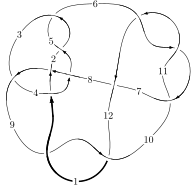
\includegraphics[width=112pt]{../../../GIT/diagram.site/Diagrams/png/1650_12a_0849.png}\\
\ \ \ A knot diagram\footnotemark}&
\allowdisplaybreaks
\textbf{Linearized knot diagam} \\
\cline{2-2}
 &
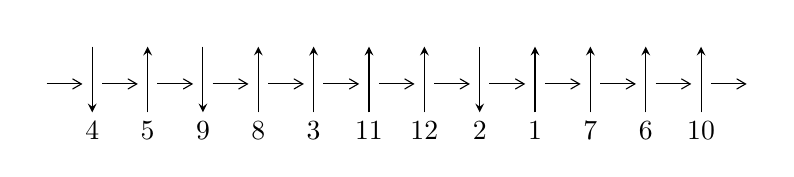
\begin{tikzpicture}[x=20pt, y=17pt]
	% nodes
	\node (C0) at (0, 0) {};
	\node (C1) at (1, 0) {};
	\node (C1U) at (1, +1) {};
	\node (C1D) at (1, -1) {4};

	\node (C2) at (2, 0) {};
	\node (C2U) at (2, +1) {};
	\node (C2D) at (2, -1) {5};

	\node (C3) at (3, 0) {};
	\node (C3U) at (3, +1) {};
	\node (C3D) at (3, -1) {9};

	\node (C4) at (4, 0) {};
	\node (C4U) at (4, +1) {};
	\node (C4D) at (4, -1) {8};

	\node (C5) at (5, 0) {};
	\node (C5U) at (5, +1) {};
	\node (C5D) at (5, -1) {3};

	\node (C6) at (6, 0) {};
	\node (C6U) at (6, +1) {};
	\node (C6D) at (6, -1) {11};

	\node (C7) at (7, 0) {};
	\node (C7U) at (7, +1) {};
	\node (C7D) at (7, -1) {12};

	\node (C8) at (8, 0) {};
	\node (C8U) at (8, +1) {};
	\node (C8D) at (8, -1) {2};

	\node (C9) at (9, 0) {};
	\node (C9U) at (9, +1) {};
	\node (C9D) at (9, -1) {1};

	\node (C10) at (10, 0) {};
	\node (C10U) at (10, +1) {};
	\node (C10D) at (10, -1) {7};

	\node (C11) at (11, 0) {};
	\node (C11U) at (11, +1) {};
	\node (C11D) at (11, -1) {6};

	\node (C12) at (12, 0) {};
	\node (C12U) at (12, +1) {};
	\node (C12D) at (12, -1) {10};
	\node (C13) at (13, 0) {};

	% arrows
	\draw[->,>={angle 60}]
	(C0) edge (C1) (C1) edge (C2) (C2) edge (C3) (C3) edge (C4) (C4) edge (C5) (C5) edge (C6) (C6) edge (C7) (C7) edge (C8) (C8) edge (C9) (C9) edge (C10) (C10) edge (C11) (C11) edge (C12) (C12) edge (C13) ;	\draw[->,>=stealth]
	(C1U) edge (C1D) (C2D) edge (C2U) (C3U) edge (C3D) (C4D) edge (C4U) (C5D) edge (C5U) (C6D) edge (C6U) (C7D) edge (C7U) (C8U) edge (C8D) (C9D) edge (C9U) (C10D) edge (C10U) (C11D) edge (C11U) (C12D) edge (C12U) ;
	\end{tikzpicture} \\
\hhline{~~} \\& 
\textbf{Solving Sequence} \\ \cline{2-2} 
 &
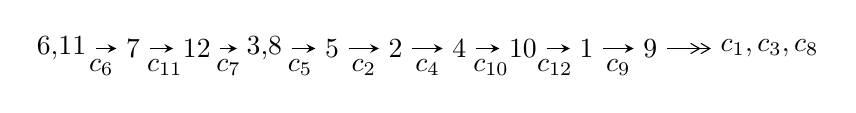
\begin{tikzpicture}[x=23pt, y=7pt]
	% node
	\node (A0) at (-1/8, 0) {6,11};
	\node (A1) at (1, 0) {7};
	\node (A2) at (2, 0) {12};
	\node (A3) at (49/16, 0) {3,8};
	\node (A4) at (33/8, 0) {5};
	\node (A5) at (41/8, 0) {2};
	\node (A6) at (49/8, 0) {4};
	\node (A7) at (57/8, 0) {10};
	\node (A8) at (65/8, 0) {1};
	\node (A9) at (73/8, 0) {9};
	\node (C1) at (1/2, -1) {$c_{6}$};
	\node (C2) at (3/2, -1) {$c_{11}$};
	\node (C3) at (5/2, -1) {$c_{7}$};
	\node (C4) at (29/8, -1) {$c_{5}$};
	\node (C5) at (37/8, -1) {$c_{2}$};
	\node (C6) at (45/8, -1) {$c_{4}$};
	\node (C7) at (53/8, -1) {$c_{10}$};
	\node (C8) at (61/8, -1) {$c_{12}$};
	\node (C9) at (69/8, -1) {$c_{9}$};
	\node (A10) at (11, 0) {$c_{1},c_{3},c_{8}$};

	% edge
	\draw[->,>=stealth]	
	(A0) edge (A1) (A1) edge (A2) (A2) edge (A3) (A3) edge (A4) (A4) edge (A5) (A5) edge (A6) (A6) edge (A7) (A7) edge (A8) (A8) edge (A9) ;
	\draw[->>,>={angle 60}]	
	(A9) edge (A10);
\end{tikzpicture} \\ 

\end{tabular} \\

\footnotetext{
The image of knot diagram is generated by the software ``\textbf{Draw programme}" developed by Andrew Bartholomew(\url{http://www.layer8.co.uk/maths/draw/index.htm\#Running-draw}), where we modified some parts for our purpose(\url{https://github.com/CATsTAILs/LinksPainter}).
}\phantom \\ \newline 
\centering \textbf{Ideals for irreducible components\footnotemark of $X_{\text{par}}$} 
 
\begin{align*}
I^u_{1}&=\langle 
1.32931\times10^{30} u^{95}+1.20412\times10^{30} u^{94}+\cdots+7.27256\times10^{30} b+8.60188\times10^{30},\\
\phantom{I^u_{1}}&\phantom{= \langle  }-5.06565\times10^{31} u^{95}-6.53663\times10^{31} u^{94}+\cdots+7.27256\times10^{30} a-1.00027\times10^{32},\;u^{96}+2 u^{95}+\cdots+7 u+1\rangle \\
I^u_{2}&=\langle 
b-1,\;2 u^2+a+2 u+4,\;u^3+u^2+2 u+1\rangle \\
\\
\end{align*}
\raggedright * 2 irreducible components of $\dim_{\mathbb{C}}=0$, with total 99 representations.\\
\footnotetext{All coefficients of polynomials are rational numbers. But the coefficients are sometimes approximated in decimal forms when there is not enough margin.}
\newpage
\renewcommand{\arraystretch}{1}
\centering \section*{I. $I^u_{1}= \langle 1.33\times10^{30} u^{95}+1.20\times10^{30} u^{94}+\cdots+7.27\times10^{30} b+8.60\times10^{30},\;-5.07\times10^{31} u^{95}-6.54\times10^{31} u^{94}+\cdots+7.27\times10^{30} a-1.00\times10^{32},\;u^{96}+2 u^{95}+\cdots+7 u+1 \rangle$}
\flushleft \textbf{(i) Arc colorings}\\
\begin{tabular}{m{7pt} m{180pt} m{7pt} m{180pt} }
\flushright $a_{6}=$&$\begin{pmatrix}1\\0\end{pmatrix}$ \\
\flushright $a_{11}=$&$\begin{pmatrix}0\\u\end{pmatrix}$ \\
\flushright $a_{7}=$&$\begin{pmatrix}1\\- u^2\end{pmatrix}$ \\
\flushright $a_{12}=$&$\begin{pmatrix}u\\u\end{pmatrix}$ \\
\flushright $a_{3}=$&$\begin{pmatrix}6.96543 u^{95}+8.98808 u^{94}+\cdots+78.9927 u+13.7540\\-0.182784 u^{95}-0.165570 u^{94}+\cdots-1.10810 u-1.18279\end{pmatrix}$ \\
\flushright $a_{8}=$&$\begin{pmatrix}- u^4- u^2+1\\- u^4-2 u^2\end{pmatrix}$ \\
\flushright $a_{5}=$&$\begin{pmatrix}-6.95549 u^{95}-8.88213 u^{94}+\cdots-78.9211 u-12.8011\\0.268862 u^{95}+0.337722 u^{94}+\cdots+1.56759 u+1.26886\end{pmatrix}$ \\
\flushright $a_{2}=$&$\begin{pmatrix}-0.202655 u^{95}+0.622541 u^{94}+\cdots+0.748795 u+0.911274\\0.827844 u^{95}+1.65570 u^{94}+\cdots+5.08103 u+0.827852\end{pmatrix}$ \\
\flushright $a_{4}=$&$\begin{pmatrix}-5.15923 u^{95}-6.25695 u^{94}+\cdots-50.6792 u-7.80846\\-1.49853 u^{95}-1.59703 u^{94}+\cdots-10.8403 u-1.49850\end{pmatrix}$ \\
\flushright $a_{10}=$&$\begin{pmatrix}- u\\u^3+u\end{pmatrix}$ \\
\flushright $a_{1}=$&$\begin{pmatrix}u^5+2 u^3+u\\- u^7-3 u^5-2 u^3+u\end{pmatrix}$ \\
\flushright $a_{9}=$&$\begin{pmatrix}- u^9-4 u^7-5 u^5-2 u^3- u\\u^{11}+5 u^9+8 u^7+3 u^5- u^3+u\end{pmatrix}$\\&\end{tabular}
\flushleft \textbf{(ii) Obstruction class $= -1$}\\~\\
\flushleft \textbf{(iii) Cusp Shapes $= -44.5807 u^{95}-59.4013 u^{94}+\cdots-458.070 u-89.9807$}\\~\\
\newpage\renewcommand{\arraystretch}{1}
\flushleft \textbf{(iv) u-Polynomials at the component}\newline \\
\begin{tabular}{m{50pt}|m{274pt}}
Crossings & \hspace{64pt}u-Polynomials at each crossing \\
\hline $$\begin{aligned}c_{1}\end{aligned}$$&$\begin{aligned}
&u^{96}-15 u^{95}+\cdots+20 u+8
\end{aligned}$\\
\hline $$\begin{aligned}c_{2},c_{5}\end{aligned}$$&$\begin{aligned}
&u^{96}+4 u^{95}+\cdots+10 u-1
\end{aligned}$\\
\hline $$\begin{aligned}c_{3}\end{aligned}$$&$\begin{aligned}
&u^{96}- u^{95}+\cdots-3474 u-1117
\end{aligned}$\\
\hline $$\begin{aligned}c_{4}\end{aligned}$$&$\begin{aligned}
&u^{96}-3 u^{95}+\cdots-2 u+1
\end{aligned}$\\
\hline $$\begin{aligned}c_{6},c_{10},c_{11}\end{aligned}$$&$\begin{aligned}
&u^{96}-2 u^{95}+\cdots-7 u+1
\end{aligned}$\\
\hline $$\begin{aligned}c_{7}\end{aligned}$$&$\begin{aligned}
&u^{96}+2 u^{95}+\cdots-38535 u+4113
\end{aligned}$\\
\hline $$\begin{aligned}c_{8}\end{aligned}$$&$\begin{aligned}
&u^{96}+4 u^{95}+\cdots- u-1
\end{aligned}$\\
\hline $$\begin{aligned}c_{9},c_{12}\end{aligned}$$&$\begin{aligned}
&u^{96}+14 u^{95}+\cdots+1779 u+99
\end{aligned}$\\
\hline
\end{tabular}\\~\\
\newpage\renewcommand{\arraystretch}{1}
\flushleft \textbf{(v) Riley Polynomials at the component}\newline \\
\begin{tabular}{m{50pt}|m{274pt}}
Crossings & \hspace{64pt}Riley Polynomials at each crossing \\
\hline $$\begin{aligned}c_{1}\end{aligned}$$&$\begin{aligned}
&y^{96}-21 y^{95}+\cdots-1360 y+64
\end{aligned}$\\
\hline $$\begin{aligned}c_{2},c_{5}\end{aligned}$$&$\begin{aligned}
&y^{96}-56 y^{95}+\cdots-94 y+1
\end{aligned}$\\
\hline $$\begin{aligned}c_{3}\end{aligned}$$&$\begin{aligned}
&y^{96}-99 y^{95}+\cdots-48978824 y+1247689
\end{aligned}$\\
\hline $$\begin{aligned}c_{4}\end{aligned}$$&$\begin{aligned}
&y^{96}-87 y^{95}+\cdots-252 y+1
\end{aligned}$\\
\hline $$\begin{aligned}c_{6},c_{10},c_{11}\end{aligned}$$&$\begin{aligned}
&y^{96}+90 y^{95}+\cdots- y+1
\end{aligned}$\\
\hline $$\begin{aligned}c_{7}\end{aligned}$$&$\begin{aligned}
&y^{96}+34 y^{95}+\cdots+341340939 y+16916769
\end{aligned}$\\
\hline $$\begin{aligned}c_{8}\end{aligned}$$&$\begin{aligned}
&y^{96}+14 y^{95}+\cdots- y+1
\end{aligned}$\\
\hline $$\begin{aligned}c_{9},c_{12}\end{aligned}$$&$\begin{aligned}
&y^{96}+82 y^{95}+\cdots+834363 y+9801
\end{aligned}$\\
\hline
\end{tabular}\\~\\
\newpage\flushleft \textbf{(vi) Complex Volumes and Cusp Shapes}
$$\begin{array}{c|c|c}  
\text{Solutions to }I^u_{1}& \I (\text{vol} + \sqrt{-1}CS) & \text{Cusp shape}\\
 \hline 
\begin{aligned}
u &= \phantom{-}0.153003 + 1.008460 I \\
a &= -0.271535 + 0.072599 I \\
b &= \phantom{-}1.206140 - 0.396842 I\end{aligned}
 & \phantom{-}1.96795 - 5.00766 I & \phantom{-0.000000 } 0 \\ \hline\begin{aligned}
u &= \phantom{-}0.153003 - 1.008460 I \\
a &= -0.271535 - 0.072599 I \\
b &= \phantom{-}1.206140 + 0.396842 I\end{aligned}
 & \phantom{-}1.96795 + 5.00766 I & \phantom{-0.000000 } 0 \\ \hline\begin{aligned}
u &= -0.703444 + 0.408687 I \\
a &= -0.91970 - 2.11043 I \\
b &= \phantom{-}1.31214 - 0.62793 I\end{aligned}
 & -1.73503 - 13.84140 I & \phantom{-0.000000 -}0. + 9.67099 I \\ \hline\begin{aligned}
u &= -0.703444 - 0.408687 I \\
a &= -0.91970 + 2.11043 I \\
b &= \phantom{-}1.31214 + 0.62793 I\end{aligned}
 & -1.73503 + 13.84140 I & \phantom{-0.000000 } 0. - 9.67099 I \\ \hline\begin{aligned}
u &= \phantom{-}0.632884 + 0.499159 I \\
a &= -0.268709 + 0.706768 I \\
b &= \phantom{-}0.518532 + 0.413160 I\end{aligned}
 & -4.70766 + 1.90436 I & \phantom{-0.000000 } 0 \\ \hline\begin{aligned}
u &= \phantom{-}0.632884 - 0.499159 I \\
a &= -0.268709 - 0.706768 I \\
b &= \phantom{-}0.518532 - 0.413160 I\end{aligned}
 & -4.70766 - 1.90436 I & \phantom{-0.000000 } 0 \\ \hline\begin{aligned}
u &= -0.587460 + 0.551315 I \\
a &= \phantom{-}0.372753 + 0.400441 I \\
b &= \phantom{-}1.28577 + 0.62488 I\end{aligned}
 & -2.27074 + 9.51260 I & \phantom{-0.000000 } 0 \\ \hline\begin{aligned}
u &= -0.587460 - 0.551315 I \\
a &= \phantom{-}0.372753 - 0.400441 I \\
b &= \phantom{-}1.28577 - 0.62488 I\end{aligned}
 & -2.27074 - 9.51260 I & \phantom{-0.000000 } 0 \\ \hline\begin{aligned}
u &= \phantom{-}0.668900 + 0.448574 I \\
a &= \phantom{-}0.236104 - 0.000583 I \\
b &= \phantom{-}0.415949 - 0.413487 I\end{aligned}
 & -4.52666 + 2.41894 I & \phantom{-0.000000 } 0 \\ \hline\begin{aligned}
u &= \phantom{-}0.668900 - 0.448574 I \\
a &= \phantom{-}0.236104 + 0.000583 I \\
b &= \phantom{-}0.415949 + 0.413487 I\end{aligned}
 & -4.52666 - 2.41894 I & \phantom{-0.000000 } 0\\
 \hline 
 \end{array}$$\newpage$$\begin{array}{c|c|c}  
\text{Solutions to }I^u_{1}& \I (\text{vol} + \sqrt{-1}CS) & \text{Cusp shape}\\
 \hline 
\begin{aligned}
u &= \phantom{-}0.702362 + 0.390466 I \\
a &= -1.03144 + 1.45734 I \\
b &= \phantom{-}0.973713 + 0.422095 I\end{aligned}
 & -3.01891 + 6.06655 I & \phantom{-}6.00000 - 8.45994 I \\ \hline\begin{aligned}
u &= \phantom{-}0.702362 - 0.390466 I \\
a &= -1.03144 - 1.45734 I \\
b &= \phantom{-}0.973713 - 0.422095 I\end{aligned}
 & -3.01891 - 6.06655 I & \phantom{-}6.00000 + 8.45994 I \\ \hline\begin{aligned}
u &= -0.204748 + 0.773490 I \\
a &= -0.174383 - 0.537365 I \\
b &= \phantom{-}1.142260 - 0.379821 I\end{aligned}
 & \phantom{-}1.82630 - 5.03644 I & \phantom{-}6.00000 + 7.08141 I \\ \hline\begin{aligned}
u &= -0.204748 - 0.773490 I \\
a &= -0.174383 + 0.537365 I \\
b &= \phantom{-}1.142260 + 0.379821 I\end{aligned}
 & \phantom{-}1.82630 + 5.03644 I & \phantom{-}6.00000 - 7.08141 I \\ \hline\begin{aligned}
u &= -0.673350 + 0.420505 I \\
a &= \phantom{-}1.196640 + 0.660554 I \\
b &= \phantom{-}0.196897 + 1.192440 I\end{aligned}
 & -5.26476 - 7.49346 I & \phantom{-0.000000 -}0. + 8.18355 I \\ \hline\begin{aligned}
u &= -0.673350 - 0.420505 I \\
a &= \phantom{-}1.196640 - 0.660554 I \\
b &= \phantom{-}0.196897 - 1.192440 I\end{aligned}
 & -5.26476 + 7.49346 I & \phantom{-0.000000 } 0. - 8.18355 I \\ \hline\begin{aligned}
u &= \phantom{-}0.555761 + 0.553665 I \\
a &= -0.120119 - 0.231294 I \\
b &= \phantom{-}0.904225 - 0.440262 I\end{aligned}
 & -3.65768 - 1.83252 I & \phantom{-}1.49951 + 2.23282 I \\ \hline\begin{aligned}
u &= \phantom{-}0.555761 - 0.553665 I \\
a &= -0.120119 + 0.231294 I \\
b &= \phantom{-}0.904225 + 0.440262 I\end{aligned}
 & -3.65768 + 1.83252 I & \phantom{-}1.49951 - 2.23282 I \\ \hline\begin{aligned}
u &= -0.595789 + 0.504630 I \\
a &= -0.597624 - 1.232220 I \\
b &= \phantom{-}0.234156 - 1.154180 I\end{aligned}
 & -5.60324 + 3.28204 I & \phantom{-}1.63591 - 1.83238 I \\ \hline\begin{aligned}
u &= -0.595789 - 0.504630 I \\
a &= -0.597624 + 1.232220 I \\
b &= \phantom{-}0.234156 + 1.154180 I\end{aligned}
 & -5.60324 - 3.28204 I & \phantom{-}1.63591 + 1.83238 I\\
 \hline 
 \end{array}$$\newpage$$\begin{array}{c|c|c}  
\text{Solutions to }I^u_{1}& \I (\text{vol} + \sqrt{-1}CS) & \text{Cusp shape}\\
 \hline 
\begin{aligned}
u &= \phantom{-}0.024677 + 1.240660 I \\
a &= -1.063710 + 0.371465 I \\
b &= -0.402686 + 0.659868 I\end{aligned}
 & -2.09706 - 1.50142 I & \phantom{-0.000000 } 0 \\ \hline\begin{aligned}
u &= \phantom{-}0.024677 - 1.240660 I \\
a &= -1.063710 - 0.371465 I \\
b &= -0.402686 - 0.659868 I\end{aligned}
 & -2.09706 + 1.50142 I & \phantom{-0.000000 } 0 \\ \hline\begin{aligned}
u &= \phantom{-}0.628440 + 0.422747 I \\
a &= \phantom{-}0.70391 - 3.17518 I \\
b &= -0.978081 - 0.185709 I\end{aligned}
 & -1.52279 + 2.67235 I & \phantom{-}2.38465 + 7.06877 I \\ \hline\begin{aligned}
u &= \phantom{-}0.628440 - 0.422747 I \\
a &= \phantom{-}0.70391 + 3.17518 I \\
b &= -0.978081 + 0.185709 I\end{aligned}
 & -1.52279 - 2.67235 I & \phantom{-}2.38465 - 7.06877 I \\ \hline\begin{aligned}
u &= -0.641923 + 0.400628 I \\
a &= \phantom{-}0.68898 + 2.25835 I \\
b &= -1.18079 + 0.83093 I\end{aligned}
 & \phantom{-}0.09155 - 5.48475 I & \phantom{-}8.75594 + 9.17307 I \\ \hline\begin{aligned}
u &= -0.641923 - 0.400628 I \\
a &= \phantom{-}0.68898 - 2.25835 I \\
b &= -1.18079 - 0.83093 I\end{aligned}
 & \phantom{-}0.09155 + 5.48475 I & \phantom{-}8.75594 - 9.17307 I \\ \hline\begin{aligned}
u &= \phantom{-}0.126353 + 1.244880 I \\
a &= \phantom{-}0.007578 - 0.630595 I \\
b &= -1.44171 + 0.35254 I\end{aligned}
 & \phantom{-}0.877763 + 0.830502 I & \phantom{-0.000000 } 0 \\ \hline\begin{aligned}
u &= \phantom{-}0.126353 - 1.244880 I \\
a &= \phantom{-}0.007578 + 0.630595 I \\
b &= -1.44171 - 0.35254 I\end{aligned}
 & \phantom{-}0.877763 - 0.830502 I & \phantom{-0.000000 } 0 \\ \hline\begin{aligned}
u &= \phantom{-}0.600345 + 0.445280 I \\
a &= -0.07428 + 1.54911 I \\
b &= -0.932084 + 0.194970 I\end{aligned}
 & -1.63276 + 1.32893 I & \phantom{-}3.90509 - 12.70354 I \\ \hline\begin{aligned}
u &= \phantom{-}0.600345 - 0.445280 I \\
a &= -0.07428 - 1.54911 I \\
b &= -0.932084 - 0.194970 I\end{aligned}
 & -1.63276 - 1.32893 I & \phantom{-}3.90509 + 12.70354 I\\
 \hline 
 \end{array}$$\newpage$$\begin{array}{c|c|c}  
\text{Solutions to }I^u_{1}& \I (\text{vol} + \sqrt{-1}CS) & \text{Cusp shape}\\
 \hline 
\begin{aligned}
u &= -0.256255 + 1.232760 I \\
a &= -0.695900 - 0.825623 I \\
b &= \phantom{-}0.840998 - 0.142886 I\end{aligned}
 & -1.81624 - 3.46446 I & \phantom{-0.000000 } 0 \\ \hline\begin{aligned}
u &= -0.256255 - 1.232760 I \\
a &= -0.695900 + 0.825623 I \\
b &= \phantom{-}0.840998 + 0.142886 I\end{aligned}
 & -1.81624 + 3.46446 I & \phantom{-0.000000 } 0 \\ \hline\begin{aligned}
u &= -0.565635 + 0.455915 I \\
a &= -1.076150 - 0.472763 I \\
b &= -1.092730 - 0.817335 I\end{aligned}
 & -0.19466 + 1.54393 I & \phantom{-}7.56354 - 2.53910 I \\ \hline\begin{aligned}
u &= -0.565635 - 0.455915 I \\
a &= -1.076150 + 0.472763 I \\
b &= -1.092730 + 0.817335 I\end{aligned}
 & -0.19466 - 1.54393 I & \phantom{-}7.56354 + 2.53910 I \\ \hline\begin{aligned}
u &= -0.697603 + 0.194178 I \\
a &= -0.968545 - 1.013010 I \\
b &= \phantom{-}1.096860 + 0.277903 I\end{aligned}
 & \phantom{-}3.87528 + 1.50507 I & \phantom{-}10.52753 - 4.31904 I \\ \hline\begin{aligned}
u &= -0.697603 - 0.194178 I \\
a &= -0.968545 + 1.013010 I \\
b &= \phantom{-}1.096860 - 0.277903 I\end{aligned}
 & \phantom{-}3.87528 - 1.50507 I & \phantom{-}10.52753 + 4.31904 I \\ \hline\begin{aligned}
u &= -0.595029 + 0.396930 I \\
a &= -0.08683 + 1.50601 I \\
b &= -1.58195 - 0.06129 I\end{aligned}
 & \phantom{-}1.52959 - 1.86728 I & \phantom{-}10.94638 + 3.68908 I \\ \hline\begin{aligned}
u &= -0.595029 - 0.396930 I \\
a &= -0.08683 - 1.50601 I \\
b &= -1.58195 + 0.06129 I\end{aligned}
 & \phantom{-}1.52959 + 1.86728 I & \phantom{-}10.94638 - 3.68908 I \\ \hline\begin{aligned}
u &= \phantom{-}0.167705 + 1.274520 I \\
a &= \phantom{-}0.53562 - 2.04164 I \\
b &= -1.32435 - 0.59778 I\end{aligned}
 & \phantom{-}0.41925 + 4.34629 I & \phantom{-0.000000 } 0 \\ \hline\begin{aligned}
u &= \phantom{-}0.167705 - 1.274520 I \\
a &= \phantom{-}0.53562 + 2.04164 I \\
b &= -1.32435 + 0.59778 I\end{aligned}
 & \phantom{-}0.41925 - 4.34629 I & \phantom{-0.000000 } 0\\
 \hline 
 \end{array}$$\newpage$$\begin{array}{c|c|c}  
\text{Solutions to }I^u_{1}& \I (\text{vol} + \sqrt{-1}CS) & \text{Cusp shape}\\
 \hline 
\begin{aligned}
u &= -0.133842 + 1.293040 I \\
a &= \phantom{-}3.29894 + 3.32621 I \\
b &= -1.038190 + 0.051286 I\end{aligned}
 & -1.42201 - 2.22010 I & \phantom{-0.000000 } 0 \\ \hline\begin{aligned}
u &= -0.133842 - 1.293040 I \\
a &= \phantom{-}3.29894 - 3.32621 I \\
b &= -1.038190 - 0.051286 I\end{aligned}
 & -1.42201 + 2.22010 I & \phantom{-0.000000 } 0 \\ \hline\begin{aligned}
u &= -0.072444 + 1.299150 I \\
a &= -1.72774 - 0.95900 I \\
b &= -0.628389 + 0.021669 I\end{aligned}
 & -2.36624 - 1.57306 I & \phantom{-0.000000 } 0 \\ \hline\begin{aligned}
u &= -0.072444 - 1.299150 I \\
a &= -1.72774 + 0.95900 I \\
b &= -0.628389 - 0.021669 I\end{aligned}
 & -2.36624 + 1.57306 I & \phantom{-0.000000 } 0 \\ \hline\begin{aligned}
u &= \phantom{-}0.684163 + 0.124406 I \\
a &= -1.98358 + 0.70879 I \\
b &= \phantom{-}1.260670 + 0.460630 I\end{aligned}
 & \phantom{-}4.61639 + 8.36713 I & \phantom{-}11.15155 - 8.05320 I \\ \hline\begin{aligned}
u &= \phantom{-}0.684163 - 0.124406 I \\
a &= -1.98358 - 0.70879 I \\
b &= \phantom{-}1.260670 - 0.460630 I\end{aligned}
 & \phantom{-}4.61639 - 8.36713 I & \phantom{-}11.15155 + 8.05320 I \\ \hline\begin{aligned}
u &= -0.695074\phantom{ +0.000000I} \\
a &= -1.61590\phantom{ +0.000000I} \\
b &= \phantom{-}0.785601\phantom{ +0.000000I}\end{aligned}
 & \phantom{-}1.96527\phantom{ +0.000000I} & -0.636190\phantom{ +0.000000I} \\ \hline\begin{aligned}
u &= \phantom{-}0.254305 + 1.300410 I \\
a &= -0.57383 + 1.87834 I \\
b &= \phantom{-}1.292740 + 0.501209 I\end{aligned}
 & \phantom{-}0.18064 + 11.76790 I & \phantom{-0.000000 } 0 \\ \hline\begin{aligned}
u &= \phantom{-}0.254305 - 1.300410 I \\
a &= -0.57383 - 1.87834 I \\
b &= \phantom{-}1.292740 - 0.501209 I\end{aligned}
 & \phantom{-}0.18064 - 11.76790 I & \phantom{-0.000000 } 0 \\ \hline\begin{aligned}
u &= \phantom{-}0.198121 + 1.315590 I \\
a &= \phantom{-}0.758091 - 0.936718 I \\
b &= -0.028658 - 1.022200 I\end{aligned}
 & -3.87109 + 6.49061 I & \phantom{-0.000000 } 0\\
 \hline 
 \end{array}$$\newpage$$\begin{array}{c|c|c}  
\text{Solutions to }I^u_{1}& \I (\text{vol} + \sqrt{-1}CS) & \text{Cusp shape}\\
 \hline 
\begin{aligned}
u &= \phantom{-}0.198121 - 1.315590 I \\
a &= \phantom{-}0.758091 + 0.936718 I \\
b &= -0.028658 + 1.022200 I\end{aligned}
 & -3.87109 - 6.49061 I & \phantom{-0.000000 } 0 \\ \hline\begin{aligned}
u &= -0.152128 + 1.326590 I \\
a &= -0.628567 + 0.511251 I \\
b &= -0.056517 + 0.160373 I\end{aligned}
 & -3.38330 - 2.54068 I & \phantom{-0.000000 } 0 \\ \hline\begin{aligned}
u &= -0.152128 - 1.326590 I \\
a &= -0.628567 - 0.511251 I \\
b &= -0.056517 - 0.160373 I\end{aligned}
 & -3.38330 + 2.54068 I & \phantom{-0.000000 } 0 \\ \hline\begin{aligned}
u &= -0.275376 + 1.354110 I \\
a &= \phantom{-}0.312578 - 0.885221 I \\
b &= \phantom{-}1.047910 + 0.215453 I\end{aligned}
 & -1.00281 - 2.01992 I & \phantom{-0.000000 } 0 \\ \hline\begin{aligned}
u &= -0.275376 - 1.354110 I \\
a &= \phantom{-}0.312578 + 0.885221 I \\
b &= \phantom{-}1.047910 - 0.215453 I\end{aligned}
 & -1.00281 + 2.01992 I & \phantom{-0.000000 } 0 \\ \hline\begin{aligned}
u &= \phantom{-}0.029052 + 1.401310 I \\
a &= -0.16252 + 1.51915 I \\
b &= \phantom{-}0.405032 + 0.751976 I\end{aligned}
 & -6.87743 - 0.86326 I & \phantom{-0.000000 } 0 \\ \hline\begin{aligned}
u &= \phantom{-}0.029052 - 1.401310 I \\
a &= -0.16252 - 1.51915 I \\
b &= \phantom{-}0.405032 - 0.751976 I\end{aligned}
 & -6.87743 + 0.86326 I & \phantom{-0.000000 } 0 \\ \hline\begin{aligned}
u &= \phantom{-}0.580873 + 0.136352 I \\
a &= \phantom{-}0.375506 + 0.481129 I \\
b &= -0.073272 - 0.878443 I\end{aligned}
 & \phantom{-}0.64889 + 3.65142 I & \phantom{-}8.61986 - 8.48689 I \\ \hline\begin{aligned}
u &= \phantom{-}0.580873 - 0.136352 I \\
a &= \phantom{-}0.375506 - 0.481129 I \\
b &= -0.073272 + 0.878443 I\end{aligned}
 & \phantom{-}0.64889 - 3.65142 I & \phantom{-}8.61986 + 8.48689 I \\ \hline\begin{aligned}
u &= \phantom{-}0.568402 + 0.038675 I \\
a &= \phantom{-}2.43556 - 0.29965 I \\
b &= -1.33753 - 0.46810 I\end{aligned}
 & \phantom{-}4.43426 + 1.67256 I & \phantom{-}17.8731 - 4.5521 I\\
 \hline 
 \end{array}$$\newpage$$\begin{array}{c|c|c}  
\text{Solutions to }I^u_{1}& \I (\text{vol} + \sqrt{-1}CS) & \text{Cusp shape}\\
 \hline 
\begin{aligned}
u &= \phantom{-}0.568402 - 0.038675 I \\
a &= \phantom{-}2.43556 + 0.29965 I \\
b &= -1.33753 + 0.46810 I\end{aligned}
 & \phantom{-}4.43426 - 1.67256 I & \phantom{-}17.8731 + 4.5521 I \\ \hline\begin{aligned}
u &= -0.02900 + 1.45074 I \\
a &= \phantom{-}1.07846 - 1.03937 I \\
b &= \phantom{-}1.062590 - 0.502423 I\end{aligned}
 & -4.91037 - 5.54307 I & \phantom{-0.000000 } 0 \\ \hline\begin{aligned}
u &= -0.02900 - 1.45074 I \\
a &= \phantom{-}1.07846 + 1.03937 I \\
b &= \phantom{-}1.062590 + 0.502423 I\end{aligned}
 & -4.91037 + 5.54307 I & \phantom{-0.000000 } 0 \\ \hline\begin{aligned}
u &= -0.22522 + 1.45170 I \\
a &= -1.55520 + 1.27952 I \\
b &= -1.65329 - 0.07886 I\end{aligned}
 & -4.41641 - 4.89650 I & \phantom{-0.000000 } 0 \\ \hline\begin{aligned}
u &= -0.22522 - 1.45170 I \\
a &= -1.55520 - 1.27952 I \\
b &= -1.65329 + 0.07886 I\end{aligned}
 & -4.41641 + 4.89650 I & \phantom{-0.000000 } 0 \\ \hline\begin{aligned}
u &= -0.20875 + 1.46039 I \\
a &= -1.96107 - 1.24412 I \\
b &= -1.057840 - 0.893839 I\end{aligned}
 & -6.33820 - 1.30367 I & \phantom{-0.000000 } 0 \\ \hline\begin{aligned}
u &= -0.20875 - 1.46039 I \\
a &= -1.96107 + 1.24412 I \\
b &= -1.057840 + 0.893839 I\end{aligned}
 & -6.33820 + 1.30367 I & \phantom{-0.000000 } 0 \\ \hline\begin{aligned}
u &= -0.23879 + 1.45754 I \\
a &= -0.41795 + 2.92896 I \\
b &= -1.20627 + 0.87760 I\end{aligned}
 & -5.89231 - 8.71118 I & \phantom{-0.000000 } 0 \\ \hline\begin{aligned}
u &= -0.23879 - 1.45754 I \\
a &= -0.41795 - 2.92896 I \\
b &= -1.20627 - 0.87760 I\end{aligned}
 & -5.89231 + 8.71118 I & \phantom{-0.000000 } 0 \\ \hline\begin{aligned}
u &= \phantom{-}0.23154 + 1.46290 I \\
a &= -0.09303 - 3.06392 I \\
b &= -1.000560 - 0.207535 I\end{aligned}
 & -7.59739 + 5.82441 I & \phantom{-0.000000 } 0\\
 \hline 
 \end{array}$$\newpage$$\begin{array}{c|c|c}  
\text{Solutions to }I^u_{1}& \I (\text{vol} + \sqrt{-1}CS) & \text{Cusp shape}\\
 \hline 
\begin{aligned}
u &= \phantom{-}0.23154 - 1.46290 I \\
a &= -0.09303 + 3.06392 I \\
b &= -1.000560 + 0.207535 I\end{aligned}
 & -7.59739 - 5.82441 I & \phantom{-0.000000 } 0 \\ \hline\begin{aligned}
u &= \phantom{-}0.21930 + 1.46489 I \\
a &= -0.93533 + 1.57380 I \\
b &= -0.923370 + 0.234801 I\end{aligned}
 & -7.78037 + 4.33496 I & \phantom{-0.000000 } 0 \\ \hline\begin{aligned}
u &= \phantom{-}0.21930 - 1.46489 I \\
a &= -0.93533 - 1.57380 I \\
b &= -0.923370 - 0.234801 I\end{aligned}
 & -7.78037 - 4.33496 I & \phantom{-0.000000 } 0 \\ \hline\begin{aligned}
u &= \phantom{-}0.26337 + 1.46180 I \\
a &= -0.08090 + 1.89803 I \\
b &= \phantom{-}1.013180 + 0.443017 I\end{aligned}
 & -8.98436 + 9.59140 I & \phantom{-0.000000 } 0 \\ \hline\begin{aligned}
u &= \phantom{-}0.26337 - 1.46180 I \\
a &= -0.08090 - 1.89803 I \\
b &= \phantom{-}1.013180 - 0.443017 I\end{aligned}
 & -8.98436 - 9.59140 I & \phantom{-0.000000 } 0 \\ \hline\begin{aligned}
u &= -0.24762 + 1.46872 I \\
a &= \phantom{-}1.35498 + 1.75823 I \\
b &= \phantom{-}0.199257 + 1.230140 I\end{aligned}
 & -11.3587 - 10.8582 I & \phantom{-0.000000 } 0 \\ \hline\begin{aligned}
u &= -0.24762 - 1.46872 I \\
a &= \phantom{-}1.35498 - 1.75823 I \\
b &= \phantom{-}0.199257 - 1.230140 I\end{aligned}
 & -11.3587 + 10.8582 I & \phantom{-0.000000 } 0 \\ \hline\begin{aligned}
u &= -0.26124 + 1.46868 I \\
a &= \phantom{-}0.27524 - 2.66960 I \\
b &= \phantom{-}1.32483 - 0.64154 I\end{aligned}
 & -7.7879 - 17.3619 I & \phantom{-0.000000 } 0 \\ \hline\begin{aligned}
u &= -0.26124 - 1.46868 I \\
a &= \phantom{-}0.27524 + 2.66960 I \\
b &= \phantom{-}1.32483 + 0.64154 I\end{aligned}
 & -7.7879 + 17.3619 I & \phantom{-0.000000 } 0 \\ \hline\begin{aligned}
u &= \phantom{-}0.18051 + 1.48247 I \\
a &= \phantom{-}0.684881 - 0.803652 I \\
b &= \phantom{-}0.896873 - 0.524411 I\end{aligned}
 & -10.21980 + 0.79261 I & \phantom{-0.000000 } 0\\
 \hline 
 \end{array}$$\newpage$$\begin{array}{c|c|c}  
\text{Solutions to }I^u_{1}& \I (\text{vol} + \sqrt{-1}CS) & \text{Cusp shape}\\
 \hline 
\begin{aligned}
u &= \phantom{-}0.18051 - 1.48247 I \\
a &= \phantom{-}0.684881 + 0.803652 I \\
b &= \phantom{-}0.896873 + 0.524411 I\end{aligned}
 & -10.21980 - 0.79261 I & \phantom{-0.000000 } 0 \\ \hline\begin{aligned}
u &= -0.498147 + 0.084357 I \\
a &= -0.922503 + 0.449112 I \\
b &= -0.1228490 - 0.0174975 I\end{aligned}
 & \phantom{-}1.036470 - 0.221761 I & \phantom{-}10.33273 + 1.22450 I \\ \hline\begin{aligned}
u &= -0.498147 - 0.084357 I \\
a &= -0.922503 - 0.449112 I \\
b &= -0.1228490 + 0.0174975 I\end{aligned}
 & \phantom{-}1.036470 + 0.221761 I & \phantom{-}10.33273 - 1.22450 I \\ \hline\begin{aligned}
u &= -0.20394 + 1.48090 I \\
a &= -0.30491 - 2.23737 I \\
b &= \phantom{-}0.285293 - 1.169340 I\end{aligned}
 & -12.01600 + 0.38311 I & \phantom{-0.000000 } 0 \\ \hline\begin{aligned}
u &= -0.20394 - 1.48090 I \\
a &= -0.30491 + 2.23737 I \\
b &= \phantom{-}0.285293 + 1.169340 I\end{aligned}
 & -12.01600 - 0.38311 I & \phantom{-0.000000 } 0 \\ \hline\begin{aligned}
u &= \phantom{-}0.24153 + 1.47727 I \\
a &= \phantom{-}0.594461 - 0.519857 I \\
b &= \phantom{-}0.376061 - 0.477072 I\end{aligned}
 & -10.74700 + 5.74113 I & \phantom{-0.000000 } 0 \\ \hline\begin{aligned}
u &= \phantom{-}0.24153 - 1.47727 I \\
a &= \phantom{-}0.594461 + 0.519857 I \\
b &= \phantom{-}0.376061 + 0.477072 I\end{aligned}
 & -10.74700 - 5.74113 I & \phantom{-0.000000 } 0 \\ \hline\begin{aligned}
u &= -0.18777 + 1.49201 I \\
a &= \phantom{-}1.45593 + 1.03077 I \\
b &= \phantom{-}1.26730 + 0.64972 I\end{aligned}
 & -8.89539 + 6.74030 I & \phantom{-0.000000 } 0 \\ \hline\begin{aligned}
u &= -0.18777 - 1.49201 I \\
a &= \phantom{-}1.45593 - 1.03077 I \\
b &= \phantom{-}1.26730 - 0.64972 I\end{aligned}
 & -8.89539 - 6.74030 I & \phantom{-0.000000 } 0 \\ \hline\begin{aligned}
u &= \phantom{-}0.21507 + 1.48897 I \\
a &= \phantom{-}0.237376 + 1.173370 I \\
b &= \phantom{-}0.558315 + 0.491708 I\end{aligned}
 & -11.15570 + 4.98077 I & \phantom{-0.000000 } 0\\
 \hline 
 \end{array}$$\newpage$$\begin{array}{c|c|c}  
\text{Solutions to }I^u_{1}& \I (\text{vol} + \sqrt{-1}CS) & \text{Cusp shape}\\
 \hline 
\begin{aligned}
u &= \phantom{-}0.21507 - 1.48897 I \\
a &= \phantom{-}0.237376 - 1.173370 I \\
b &= \phantom{-}0.558315 - 0.491708 I\end{aligned}
 & -11.15570 - 4.98077 I & \phantom{-0.000000 } 0 \\ \hline\begin{aligned}
u &= -0.489115\phantom{ +0.000000I} \\
a &= \phantom{-}9.11251\phantom{ +0.000000I} \\
b &= -1.02527\phantom{ +0.000000I}\end{aligned}
 & \phantom{-}2.57974\phantom{ +0.000000I} & -70.0420\phantom{ +0.000000I} \\ \hline\begin{aligned}
u &= \phantom{-}0.090702 + 0.464486 I \\
a &= -0.940114 + 0.704675 I \\
b &= \phantom{-}0.127855 + 0.589477 I\end{aligned}
 & -1.16399 - 1.31134 I & -0.45702 + 1.99910 I \\ \hline\begin{aligned}
u &= \phantom{-}0.090702 - 0.464486 I \\
a &= -0.940114 - 0.704675 I \\
b &= \phantom{-}0.127855 - 0.589477 I\end{aligned}
 & -1.16399 + 1.31134 I & -0.45702 - 1.99910 I \\ \hline\begin{aligned}
u &= -0.169777 + 0.224629 I \\
a &= -2.71570 + 0.78496 I \\
b &= -1.064590 + 0.184749 I\end{aligned}
 & \phantom{-}1.94664 - 0.71724 I & \phantom{-}4.81639 - 0.29168 I \\ \hline\begin{aligned}
u &= -0.169777 - 0.224629 I \\
a &= -2.71570 - 0.78496 I \\
b &= -1.064590 - 0.184749 I\end{aligned}
 & \phantom{-}1.94664 + 0.71724 I & \phantom{-}4.81639 + 0.29168 I\\
 \hline 
 \end{array}$$\newpage\newpage\renewcommand{\arraystretch}{1}
\centering \section*{II. $I^u_{2}= \langle b-1,\;2 u^2+a+2 u+4,\;u^3+u^2+2 u+1 \rangle$}
\flushleft \textbf{(i) Arc colorings}\\
\begin{tabular}{m{7pt} m{180pt} m{7pt} m{180pt} }
\flushright $a_{6}=$&$\begin{pmatrix}1\\0\end{pmatrix}$ \\
\flushright $a_{11}=$&$\begin{pmatrix}0\\u\end{pmatrix}$ \\
\flushright $a_{7}=$&$\begin{pmatrix}1\\- u^2\end{pmatrix}$ \\
\flushright $a_{12}=$&$\begin{pmatrix}u\\u\end{pmatrix}$ \\
\flushright $a_{3}=$&$\begin{pmatrix}-2 u^2-2 u-4\\1\end{pmatrix}$ \\
\flushright $a_{8}=$&$\begin{pmatrix}- u\\- u^2- u-1\end{pmatrix}$ \\
\flushright $a_{5}=$&$\begin{pmatrix}-2 u^2-2 u-3\\1\end{pmatrix}$ \\
\flushright $a_{2}=$&$\begin{pmatrix}-1\\0\end{pmatrix}$ \\
\flushright $a_{4}=$&$\begin{pmatrix}- u^2- u-2\\0\end{pmatrix}$ \\
\flushright $a_{10}=$&$\begin{pmatrix}- u\\- u^2- u-1\end{pmatrix}$ \\
\flushright $a_{1}=$&$\begin{pmatrix}-1\\0\end{pmatrix}$ \\
\flushright $a_{9}=$&$\begin{pmatrix}u^2+1\\- u^2- u-1\end{pmatrix}$\\&\end{tabular}
\flushleft \textbf{(ii) Obstruction class $= 1$}\\~\\
\flushleft \textbf{(iii) Cusp Shapes $= 7 u^2+5 u+17$}\\~\\
\newpage\renewcommand{\arraystretch}{1}
\flushleft \textbf{(iv) u-Polynomials at the component}\newline \\
\begin{tabular}{m{50pt}|m{274pt}}
Crossings & \hspace{64pt}u-Polynomials at each crossing \\
\hline $$\begin{aligned}c_{1}\end{aligned}$$&$\begin{aligned}
&u^3
\end{aligned}$\\
\hline $$\begin{aligned}c_{2}\end{aligned}$$&$\begin{aligned}
&(u+1)^3
\end{aligned}$\\
\hline $$\begin{aligned}c_{3},c_{4}\end{aligned}$$&$\begin{aligned}
&u^3- u-1
\end{aligned}$\\
\hline $$\begin{aligned}c_{5}\end{aligned}$$&$\begin{aligned}
&(u-1)^3
\end{aligned}$\\
\hline $$\begin{aligned}c_{6}\end{aligned}$$&$\begin{aligned}
&u^3+u^2+2 u+1
\end{aligned}$\\
\hline $$\begin{aligned}c_{7},c_{8},c_{9}\end{aligned}$$&$\begin{aligned}
&u^3- u^2+1
\end{aligned}$\\
\hline $$\begin{aligned}c_{10},c_{11}\end{aligned}$$&$\begin{aligned}
&u^3- u^2+2 u-1
\end{aligned}$\\
\hline $$\begin{aligned}c_{12}\end{aligned}$$&$\begin{aligned}
&u^3+u^2-1
\end{aligned}$\\
\hline
\end{tabular}\\~\\
\newpage\renewcommand{\arraystretch}{1}
\flushleft \textbf{(v) Riley Polynomials at the component}\newline \\
\begin{tabular}{m{50pt}|m{274pt}}
Crossings & \hspace{64pt}Riley Polynomials at each crossing \\
\hline $$\begin{aligned}c_{1}\end{aligned}$$&$\begin{aligned}
&y^3
\end{aligned}$\\
\hline $$\begin{aligned}c_{2},c_{5}\end{aligned}$$&$\begin{aligned}
&(y-1)^3
\end{aligned}$\\
\hline $$\begin{aligned}c_{3},c_{4}\end{aligned}$$&$\begin{aligned}
&y^3-2 y^2+y-1
\end{aligned}$\\
\hline $$\begin{aligned}c_{6},c_{10},c_{11}\end{aligned}$$&$\begin{aligned}
&y^3+3 y^2+2 y-1
\end{aligned}$\\
\hline $$\begin{aligned}c_{7},c_{8},c_{9}\\c_{12}\end{aligned}$$&$\begin{aligned}
&y^3- y^2+2 y-1
\end{aligned}$\\
\hline
\end{tabular}\\~\\
\newpage\flushleft \textbf{(vi) Complex Volumes and Cusp Shapes}
$$\begin{array}{c|c|c}  
\text{Solutions to }I^u_{2}& \I (\text{vol} + \sqrt{-1}CS) & \text{Cusp shape}\\
 \hline 
\begin{aligned}
u &= -0.215080 + 1.307140 I \\
a &= -0.24512 - 1.48972 I \\
b &= \phantom{-}1.00000\phantom{ +0.000000I}\end{aligned}
 & -1.37919 - 2.82812 I & \phantom{-}4.28809 + 2.59975 I \\ \hline\begin{aligned}
u &= -0.215080 - 1.307140 I \\
a &= -0.24512 + 1.48972 I \\
b &= \phantom{-}1.00000\phantom{ +0.000000I}\end{aligned}
 & -1.37919 + 2.82812 I & \phantom{-}4.28809 - 2.59975 I \\ \hline\begin{aligned}
u &= -0.569840\phantom{ +0.000000I} \\
a &= -3.50976\phantom{ +0.000000I} \\
b &= \phantom{-}1.00000\phantom{ +0.000000I}\end{aligned}
 & \phantom{-}2.75839\phantom{ +0.000000I} & \phantom{-}16.4240\phantom{ +0.000000I}\\
 \hline 
 \end{array}$$\newpage
\newpage\renewcommand{\arraystretch}{1}
\centering \section*{ III. u-Polynomials}
\begin{tabular}{m{50pt}|m{274pt}}
Crossings & \hspace{64pt}u-Polynomials at each crossing \\
\hline $$\begin{aligned}c_{1}\end{aligned}$$&$\begin{aligned}
&u^3(u^{96}-15 u^{95}+\cdots+20 u+8)
\end{aligned}$\\
\hline $$\begin{aligned}c_{2}\end{aligned}$$&$\begin{aligned}
&((u+1)^3)(u^{96}+4 u^{95}+\cdots+10 u-1)
\end{aligned}$\\
\hline $$\begin{aligned}c_{3}\end{aligned}$$&$\begin{aligned}
&(u^3- u-1)(u^{96}- u^{95}+\cdots-3474 u-1117)
\end{aligned}$\\
\hline $$\begin{aligned}c_{4}\end{aligned}$$&$\begin{aligned}
&(u^3- u-1)(u^{96}-3 u^{95}+\cdots-2 u+1)
\end{aligned}$\\
\hline $$\begin{aligned}c_{5}\end{aligned}$$&$\begin{aligned}
&((u-1)^3)(u^{96}+4 u^{95}+\cdots+10 u-1)
\end{aligned}$\\
\hline $$\begin{aligned}c_{6}\end{aligned}$$&$\begin{aligned}
&(u^3+u^2+2 u+1)(u^{96}-2 u^{95}+\cdots-7 u+1)
\end{aligned}$\\
\hline $$\begin{aligned}c_{7}\end{aligned}$$&$\begin{aligned}
&(u^3- u^2+1)(u^{96}+2 u^{95}+\cdots-38535 u+4113)
\end{aligned}$\\
\hline $$\begin{aligned}c_{8}\end{aligned}$$&$\begin{aligned}
&(u^3- u^2+1)(u^{96}+4 u^{95}+\cdots- u-1)
\end{aligned}$\\
\hline $$\begin{aligned}c_{9}\end{aligned}$$&$\begin{aligned}
&(u^3- u^2+1)(u^{96}+14 u^{95}+\cdots+1779 u+99)
\end{aligned}$\\
\hline $$\begin{aligned}c_{10},c_{11}\end{aligned}$$&$\begin{aligned}
&(u^3- u^2+2 u-1)(u^{96}-2 u^{95}+\cdots-7 u+1)
\end{aligned}$\\
\hline $$\begin{aligned}c_{12}\end{aligned}$$&$\begin{aligned}
&(u^3+u^2-1)(u^{96}+14 u^{95}+\cdots+1779 u+99)
\end{aligned}$\\
\hline
\end{tabular}\newpage\renewcommand{\arraystretch}{1}
\centering \section*{ IV. Riley Polynomials}
\begin{tabular}{m{50pt}|m{274pt}}
Crossings & \hspace{64pt}Riley Polynomials at each crossing \\
\hline $$\begin{aligned}c_{1}\end{aligned}$$&$\begin{aligned}
&y^3(y^{96}-21 y^{95}+\cdots-1360 y+64)
\end{aligned}$\\
\hline $$\begin{aligned}c_{2},c_{5}\end{aligned}$$&$\begin{aligned}
&((y-1)^3)(y^{96}-56 y^{95}+\cdots-94 y+1)
\end{aligned}$\\
\hline $$\begin{aligned}c_{3}\end{aligned}$$&$\begin{aligned}
&(y^3-2 y^2+y-1)(y^{96}-99 y^{95}+\cdots-4.89788\times10^{7} y+1247689)
\end{aligned}$\\
\hline $$\begin{aligned}c_{4}\end{aligned}$$&$\begin{aligned}
&(y^3-2 y^2+y-1)(y^{96}-87 y^{95}+\cdots-252 y+1)
\end{aligned}$\\
\hline $$\begin{aligned}c_{6},c_{10},c_{11}\end{aligned}$$&$\begin{aligned}
&(y^3+3 y^2+2 y-1)(y^{96}+90 y^{95}+\cdots- y+1)
\end{aligned}$\\
\hline $$\begin{aligned}c_{7}\end{aligned}$$&$\begin{aligned}
&(y^3- y^2+2 y-1)(y^{96}+34 y^{95}+\cdots+3.41341\times10^{8} y+1.69168\times10^{7})
\end{aligned}$\\
\hline $$\begin{aligned}c_{8}\end{aligned}$$&$\begin{aligned}
&(y^3- y^2+2 y-1)(y^{96}+14 y^{95}+\cdots- y+1)
\end{aligned}$\\
\hline $$\begin{aligned}c_{9},c_{12}\end{aligned}$$&$\begin{aligned}
&(y^3- y^2+2 y-1)(y^{96}+82 y^{95}+\cdots+834363 y+9801)
\end{aligned}$\\
\hline
\end{tabular}
\vskip 2pc
\end{document}